\hideheader
\section{Εικονικοί κόσμοι \& διδασκαλία αλγορίθμων}

\subsection{Εικονικοί κόσμοι}

Ένας εικονικός κόσμος είναι ένας κοινόχρηστος, προσομοιωμένος χώρος που κατοικείται και διαμορφώνεται από τους χρήστες του, οι οποίοι αντιπροσωπεύονται ως \gls{avatar}. Τα \gls{avatar} αυτά μεσολαβούν στην εμπειρία μας σε αυτόν τον χώρο καθώς κινούμαστε, αλληλεπιδρούμε με αντικείμενα και αλληλεπιδρούμε με άλλους χρήστες, με τους οποίους διαμορφώνουμε μια κοινή κατανόηση του κόσμου εκείνη τη στιγμή.

Οι εικονικοί κόσμοι διαφέρουν από τους φυσικούς ή υλικούς κόσμους ως προς τις εμπειρίες που προσφέρουν στους χρήστες, οι οποίες διευκολύνονται από συνδυασμό τεχνικών χαρακτηριστικών, με κυριότερο το \gls{avatar}. Επίσης, χαρακτηρίζονται από τη δυνατότητα πολλαπλών ταυτόχρονων χρηστών που μπορούν να αλληλεπιδρούν μεταξύ τους σε πραγματικό χρόνο και να διαμορφώνουν το περιβάλλον γύρω τους μέσω της δημιουργίας και της διαχείρισης περιε-χομένου\cite{girvan_what_2018}.

% ========================================

\subsection{Εικονικοί κόσμοι για εκπαιδευτικούς σκοπούς}

Οι εικονικοί κόσμοι έχουν αποδειχθεί εξαιρετικά χρήσιμοι για εκπαιδευτικούς σκοπούς λόγω της ικανότητάς τους να προσφέρουν μια εμβυθιστική και διαδραστική εμπειρία μάθησης. Η ενσωμάτωση των εικονικών κόσμων στην εκπαίδευση προσφέρει πλούσιες και καινοτόμες ευκαιρίες μάθησης, βελτιώνοντας τις μαθησιακές εμπειρίες και τις επιδόσεις των μαθητών. Μερικά από τα πλεονεκτήματα των εικονικών κόσμων είναι:

\begin{itemize}
    \item \textbf{Ενίσχυση της μάθησης μέσω εμπειρίας:} Οι μαθητές μπορούν να βιώσουν καταστάσεις και φαινόμενα που θα ήταν δύσκολο ή αδύνατο να αναπαραχθούν στην πραγματική ζωή, όπως οι προσομοιώσεις φυσικών φαινομένων ή ιστορικών γεγονότων\cite{noauthor_virtual_nodate,noauthor_benefits_2019}.
    \item \textbf{Ανάπτυξη κοινωνικών δεξιοτήτων:} Μέσω της αλληλεπίδρασης με άλλους χρήστες, οι μαθητές μαθαίνουν να συνεργάζονται και να επικοινωνούν αποτελεσματικά. Οι εικονικοί κόσμοι ενισχύουν τις δεξιότητες της επικοινωνίας, της συνεργασίας, της δημιουργικότητας και της κριτικής σκέ-ψη\cite{noauthor_explore_nodate,staff_20_2022}.
    \item \textbf{Ευελιξία στη μάθηση:} Οι εικονικοί κόσμοι μπορούν να προσαρμοστούν στις ανάγκες των μαθητών, επιτρέποντας εξατομικευμένη εκπαίδευση. Επιπλέον, μπορούν να χρησιμοποιηθούν για την προσομοίωση επικίνδυνων ή αδύνατων καταστάσεων στην πραγματική ζωή, όπως η εκπαίδευση σε επικίνδυνες διαδικασίες\cite{staff_20_2022}.
    \item \textbf{Προσβασιμότητα:} Δυνατότητα συμμετοχής μαθητών από διαφορετικά γεωγραφικά σημεία, κάνοντας την εκπαίδευση πιο προσιτή και ενισχύοντας την πολιτιστική κατανόηση και την ενσυναίσθηση μέσω εικονικών ταξιδιών και εκθέσεων\cite{noauthor_virtual_nodate}.
\end{itemize}

Κάποια παραδείγματα εικονικών κόσμων είναι:

\begin{itemize}
    \item \textbf{Minecraft: Education Edition:} Αυτός ο δημοφιλής εικονικός κόσμος επιτρέπει στους μαθητές να δημιουργούν και να αλληλεπιδρούν σε ένα περιβάλλον που προάγει τη συνεργασία και την επίλυση προβλημάτων. Χρησιμοποιείται ευρέως για τη διδασκαλία διαφόρων θεμάτων, από την ιστορία έως την προγραμματιστική λογική\cite{noauthor_explore_nodate}.
    \item \textbf{Second Life:} Χρησιμοποιείται για τη διδασκαλία συγκεκριμένων επιστημονικών και τεχνικών δεξιοτήτων, όπως οι διαδικασίες αυτοψίας στην ιατροδικαστική παθολογία και η εκπαίδευση στη νοσηλευτική μέσω προσ-ομοιώσεων\cite{staff_20_2022}.
    \item \textbf{Google Expeditions:} Επιτρέπει στους μαθητές να εξερευνήσουν εικονικά ταξίδια και προορισμούς, εμπλουτίζοντας τις γνώσεις τους σε διάφορα γνωστικά πεδία, όπως η γεωμετρία και η πολιτιστική εκπαίδευση\cite{noauthor_benefits_2019}.
\end{itemize}

\begin{figure}[H]
    \centering
    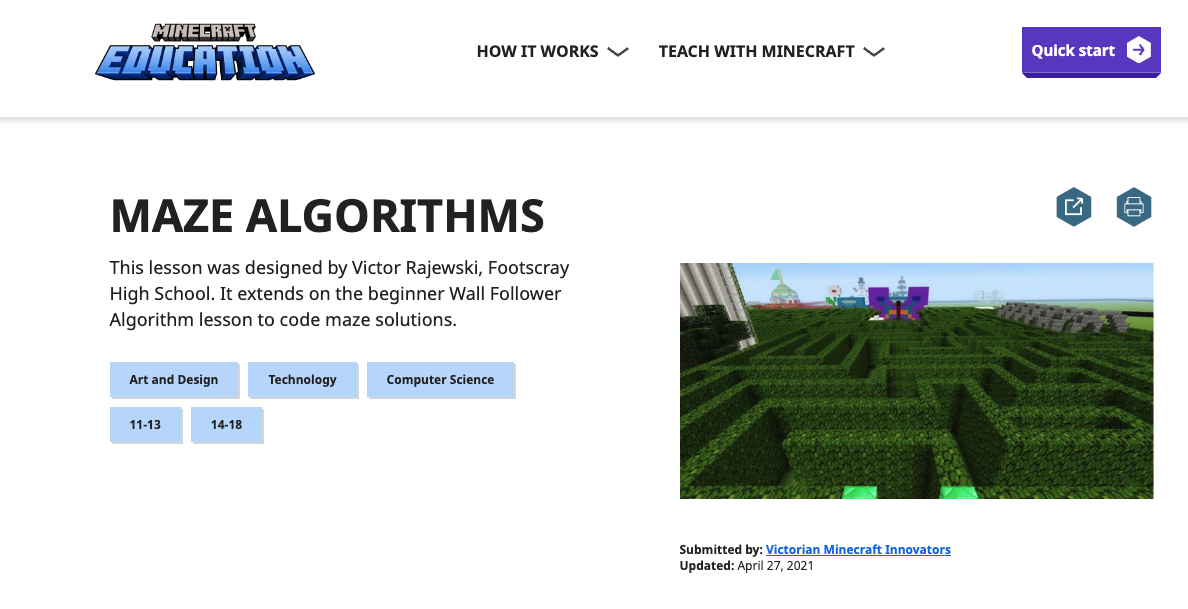
\includegraphics[width=0.8\linewidth]{sections/3/images/minecraft_edu}
    \caption{Μάθημα \underline{Maze Algorithms} στο \textbf{Minecraft: Education Edition}}
    \label{fig:minecraft_edu}
\end{figure}

Η ομάδα του εργαστηρίου \textbf{Τεχνητής νοημοσύνης και ρομποτικής} έχει αναπτύξει στο παρελθόν διάφορα εργαλεία με καινοτόμες εκπαιδευτικές προσεγγίσεις. Μία από αυτές είναι ένα εκπαιδευτικό \acrshort{3d} \acrshort{vr} περιβάλλον στο οποίο οι μαθητές αλληλεπιδρούν με \acrshort{3d} αντικείμενα, συμμετέχουν σε εικονικές τάξεις και παίρνουν μέρος σε κουίζ. Οι μαθητές είχαν τη δυνατότητα να αλληλεπιδράσουν με το περιβάλλον, λαμβάνοντας αποφάσεις βάσει των βημάτων του αλγορίθμου\cite{grivokostopoulou_innovative_2016}.

\begin{figure}[H]
    \centering
    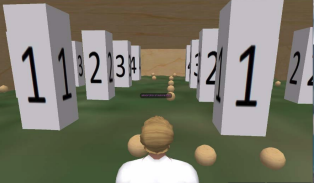
\includegraphics[width=0.8\linewidth]{sections/3/images/3d_vr}
    \caption{Ο μαθητής αλληλεπιδρά με το περιβάλλον στο εκπαιδευτικό \acrshort{3d} \acrshort{vr} περιβάλλον}
    \label{fig:3d_vr}
\end{figure}

Μία ακόμα προσέγγιση ήταν ένα εκπαιδευτικό σύστημα για τη μάθηση αλγορίθμων αναζήτησης και την αυτόματη αξιολόγηση της απόδοσης των μαθητών. Το σύστημα βασιζόταν στις αρχές της ενεργούς μάθησης και περιελάμβανε δραστηριότητες μάθησης όπως αλληλεπιδραστικές ασκήσεις και οπτικοποιήσεις α-λγορίθμων\cite{grivokostopoulou_educational_2017}.

\begin{figure}[H]
    \centering
    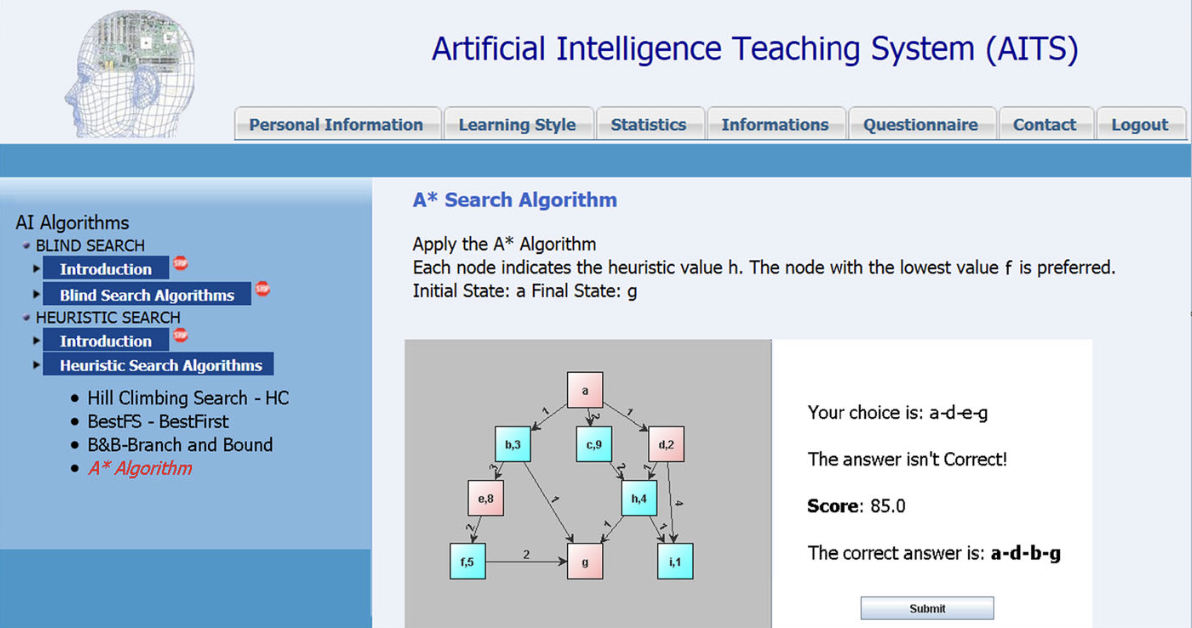
\includegraphics[width=0.8\linewidth]{sections/3/images/aits}
    \caption{Άσκηση αξιολόγησης στον αλγόριθμο \textbf{A*} στο εκπαιδευτικό σύστημα}
    \label{fig:aits}
\end{figure}

% ========================================

\subsection{Διδασκαλία αλγορίθμων σε εικονικούς κόσμους}

Η διδασκαλία αλγορίθμων σε εικονικούς κόσμους μπορεί να προσφέρει έναν καινοτόμο και αποδοτικό τρόπο για την κατανόηση και την εφαρμογή των θεμελιωδών εννοιών της πληροφορικής. Οι εικονικοί κόσμοι μπορούν να παρέχουν ένα διαδραστικό περιβάλλον όπου οι μαθητές μπορούν να πειραματιστούν με κώδικα, να δουν άμεσα τα αποτελέσματα των αλγορίθμων τους και να κατανοήσουν την επίδραση των αλλαγών που πραγματοποιούν.

Μερικά από τα πλεονεκτήματα της διδασκαλίας αλγορίθμων σε εικονικούς κόσμους περιλαμβάνουν:

\begin{itemize}
    \item \textbf{Διαδραστικότητα:} Οι μαθητές μπορούν να αλληλεπιδρούν με τα αντικείμενα του εικονικού κόσμου, επιτρέποντας την καλύτερη κατανόηση των εννοιών μέσω της πρακτικής εφαρμογής.
    \item \textbf{Άμεση ανάδραση:} Η δυνατότητα άμεσης παρατήρησης των αποτελεσμάτων των αλλαγών στον κώδικα βοηθά τους μαθητές να κατανοήσουν καλύτερα την ακολουθία των ενεργειών και την επίδρασή τους.
    \item \textbf{Οπτικοποίηση:} Οι αλγόριθμοι μπορούν να οπτικοποιηθούν με τρόπους που διευκολύνουν την κατανόηση. Για παράδειγμα, οι δομές δεδομένων μπορούν να απεικονιστούν με γραφικές παραστάσεις, και οι διεργασίες ταξινόμησης ή αναζήτησης μπορούν να παρουσιαστούν βήμα-βήμα.
    \item \textbf{Προσαρμογή και εξατομίκευση:} Οι εικονικοί κόσμοι μπορούν να προσαρμόζονται στις ανάγκες του κάθε μαθητή, παρέχοντας εξατομικευμένες ασκήσεις και προκλήσεις που αντιστοιχούν στο επίπεδο και τις δυνατότητες του κάθε ατόμου.
    \item \textbf{Συνεργασία:} Οι εικονικοί κόσμοι μπορούν να διευκολύνουν την συνεργασία μεταξύ των μαθητών, επιτρέποντας την από κοινού εργασία πάνω σε προβλήματα και την ανταλλαγή ιδεών.
    \item \textbf{Πρακτική εφαρμογή:} Οι μαθητές μπορούν να δημιουργούν και να δοκιμάζουν αλγορίθμους σε ρεαλιστικά σενάρια, ενισχύοντας την κατανόηση των εννοιών και της πρακτικής τους εφαρμογής\cite{damasevicius_virtual_2024,rossiou_using_2009}.
\end{itemize}

Για να εφαρμοστεί αποτελεσματικά η διδασκαλία αλγορίθμων σε εικονικούς κόσμους, είναι σημαντικό να υπάρχουν κατάλληλα εκπαιδευτικά εργαλεία και πλατφόρμες που να υποστηρίζουν αυτήν τη μέθοδο διδασκαλίας. Αυτά τα εργαλεία θα πρέπει να είναι προσβάσιμα, εύχρηστα και να παρέχουν επαρκή καθοδήγηση και υποστήριξη στους μαθητές.

% ========================================

\subsection{Πλατφόρμα Unity}

Η δημιουργία εικονικών κόσμων για εκπαιδευτικούς σκοπούς απαιτεί την επιλογή και χρήση εξειδικευμένων εργαλείων ανάπτυξης. Ένα από τα πιο δημοφιλή εργαλεία για τη δημιουργία εικονικών κόσμων είναι το Unity Engine.

\subsubsection{Ιστορική αναδρομή}

Το Unity Engine\cite{noauthor_real-time_nodate} είναι μια μηχανή παιχνιδιών από την Unity Technologies που κυκλοφόρησε για πρώτη φορά τον Ιούνιο του 2005. Χρησιμοποιείται ευρέως για τη δημιουργία δισδιάστατων (\acrshort{2d}) και τρισδιάστατων (\acrshort{3d}) εικονικών κόσμων, καθώς και για προσομοιώσεις και άλλες διαδραστικές εμπειρίες. Μία από τις βασικότερες πτυχές της μηχανής είναι η υποστήριξη ποικιλίας πλατφόρμων (επιτραπέζιων υπολογιστών, κινητών, κονσολών, \acrshort{ar}, \acrshort{vr}, κ.α.) κάτι το οποίο μπορεί να επιτευχθεί εύκολα, χωρίς να χρειαστεί να αλλάξει τίποτα στην υλοποίηση. Με την πάροδο του χρόνου, η μηχανή έγινε δημοφιλής μεταξύ \glspl{developer} \glspl{indie_game} και \glspl{mobile_game} λόγω της ευκολίας χρήσης και των ισχυρών εργαλείων ανάπτυξης που προσφέρει. Η ανάπτυξη εφαρμογών μέσω αυτής γίνεται με τη χρήση του Unity Editor\cite{noauthor_unity_2024,haas_history_2014}.

\subsubsection{Τρέχουσες εκδόσεις}

Από το 2017 και μετέπειτα\cite{noauthor_unity_nodate} το Unity κυκλοφορεί δύο νέες εκδόσεις του Editor κάθε χρόνο, γνωστές ως εκδόσεις \gls{tech_stream}, καθώς και μια έκδοση \acrshort{lts}. Αυτές οι εκδόσεις κυκλοφορούν συνήθως στο πρώτο και το τελευταίο τρίμηνο κάθε έτους (\gls{q1}, \gls{q4}).

Οι εκδόσεις \gls{tech_stream} προσφέρουν πρόσβαση σε όλες τις τελευταίες υπό εξέλιξη λειτουργίες και ενημερώσεις. Αυτές προορίζονται για πρωτότυπα και πειραματισμό, πριν την δέσμευση σε πλήρη ανάπτυξη έργου.

Οι εκδόσεις \acrshort{lts} υποστηρίζονται για δύο χρόνια και παρέχουν τη μέγιστη σταθερότητα και πλήρη υποστήριξη για τη δημιουργία ενός έργου. Ενημερώνονται συχνά κατά τη διάρκεια του κύκλου υποστήριξης τους, με σκοπό τη βελτίωση της απόδοσης τους και την αντιμετώπιση τυχόν προβλημάτων που χρειάζονται διόρθωση\cite{technologies_lts_nodate}.

\subsubsection{Υποστηρικτικές υπηρεσίες}

Η Unity Technologies παρέχει μια πληθώρα υπηρεσιών εκτός του Unity Engine και το Unity Editor, οι οποίες υποστηρίζουν την ανάπτυξη παιχνιδιών, την εμπορευματοποίηση και την ανάπτυξη εφαρμογών. Αυτές οι υπηρεσίες καλύπτουν διάφορες ανάγκες των προγραμματιστών και ενσωματώνονται σε διάφορα στάδια της δημιουργικής διαδικασίας. Πολλές από αυτές επίσης δεν απαιτούν την υλοποίηση μέσω Unity Editor, αλλά μπορούν να χρησιμοποιηθούν από εξωτερικές εφαρμογές και παιχνίδια. Μερικές από αυτές είναι:

\begin{itemize}
    \item \textbf{Unity Ads:} Αυτή η πλατφόρμα επιτρέπει την ενσωμάτωση διαφημίσεων στα παιχνίδια, δίνοντας τη δυνατότητα στους προγραμματιστές να έχουν άμεσα έσοδα\cite{noauthor_unity_nodate-1}.
    \item \textbf{Unity Analytics:} Παρέχει τρόπους για ανάλυση της απόδοσης του παιχνιδιού, καθώς και των συμπεριφορών των παικτών. Προσφέρει δεδομένα σε πραγματικό χρόνο καθώς και γραφήματα στατιστικών\cite{noauthor_game_nodate}.
    \item \textbf{Unity Cloud:} Υποστηρίζει την ανάπτυξη παιχνιδιών και εφαρμογών μέσω της παροχής υπηρεσιών που βελτιστοποιουν τη συνεργασία και την απόδοση της ομάδας, καθώς και μέσω υπηρεσιών για διανομή τους και υποστήριξη πολλαπλών παικτών\cite{noauthor_unity_nodate-3}.
    \item \textbf{Unity Multiplayer Services:} Είναι μέρος του Unity Cloud και προσφέρουν λύσεις για την ανάπτυξη πολυπαικτικών παιχνιδιών. Προσφέρουν hosting διακομιστών, \acrfull{sdk} για το Unity Engine, καθώς και υπηρεσίες για την κυκλοφορία και την εύρεση παικτών μέσω του δικτύου\cite{noauthor_multiplayer_nodate}.
\end{itemize}

Οι παραπάνω είναι λίγες από τις υπηρεσίες που προσφέρει η Unity Technologies. Τα προβλήματα τα οποία αυτές λύνουν έχουν ταλαιπωρήσει τον κόσμο της ανάπτυξης παιχνιδιών εδώ και χρόνια, καθώς μειώνουν το χρόνο και τη προσπάθεια που απαιτείται για τη κατασκευή και διανομή του λογισμικού\cite{al-said_ahmad_scalability_2019}.

\subsubsection{Ανταγωνιστές}

Το Unity Engine είναι μία από πιο δημοφιλείς μηχανές παιχνιδιών, αλλά υπάρχουν αρκετές ανταγωνιστικές επιλογές που προσφέρουν ποικίλα χαρακτηριστικά και πλεονεκτήματα\cite{leroux_best_2023}. Οι δημοφιλέστερες από αυτές είναι:

\begin{itemize}
    \item \textbf{Godot Engine\cite{engine_godot_nodate}:} \Gls{open_source} και δωρεάν, η Godot Engine προσφέρει ευέλικτη αρχιτεκτονική και δυνατότητες για ανάπτυξη \acrshort{2d} και \acrshort{3d} παιχνιδιών. Αποτελεί πιθανώς τον κοντινότερο ανταγωνιστή για το Unity Engine, όσον αφορά τις δυνατότητες των μηχανών.
    \item \textbf{Unreal Engine\cite{noauthor_most_nodate}:} Γνωστή για τα γραφικά υψηλής ποιότητας και την ισχυρή κοινότητα προγραμματιστών, η Unreal Engine προσφέρει δυνατότητες όπως \gls{photorealistic} \gls{rendering} και ισχυρά εργαλεία scripting με τη χρήση των Blueprints.
\end{itemize}
